
\chapter{Banaszczyk's Method }\label{ch:bana-intro}

A problem with the partial coloring method is that it requires $O(\log
n)$ rounds to obtain a full coloring, often resulting in an extra
$O(\log n)$ factor loss in the overall discrepancy bound. For example,
for the Koml\'os problem  (Problem~\ref{prob:komlos}), we incurred $O(\log n)$ discrepancy in
Exercise~\ref{ex:ch3-komlos}, even though there exists a partial
coloring with  $O(1)$ discrepancy.

In a remarkable result~\cite{Bana98}, Banaszczyk gave a different way
to find a full coloring directly, which often gives better
bounds\footnote{Though it does not seem to be directly comparable with
  the partial coloring method. For example, we do not know how to
  obtain the $O(\sqrt{n})$ for Spencer's problem using Banaszczyk's
  result}, and, in particular, improves the bound 
  %in Exercise~\ref{ex:ch3-komlos} 
to $O(\sqrt{\log n})$. 
This was the best known bound for the Koml\'os problem until very recently \cite{bansaljiang2025}.

 We now state Banaszczyk's theorem. 
 In  addition to giving an improved bound for the Koml\'os problem,
 it gives a powerful and general geometric result which has many other
 surprising applications. We  will discuss some of them in this chapter, and others later in the book. %We shall we such an example in Theorem \ref{} later.

\begin{theorem}[Banaszczyk~\cite{Bana98}]\label{thm:bana}
Let $K$ be an arbitrary closed convex set in $\mathbb{R}^m$ with Gaussian measure $\gamma^m(K)\ge 1/2$, and let $v_1,\dots,v_n\in\mathbb{R}^m$ be arbitrary vectors with length $\|v_i\|_2$  at most $1/5$. Then there exist signs $x(1),\ldots,x(n) \in \{-1,1\}$ such that $\sum_{i=1}^n x(i) v_i \in K$. 
%where $c$ is an absolute constant. In particular, $c=5$ suffices.
\end{theorem}
%Equivalently, given vectors $v_1,\ldots,v_n$ with
%$|v_i\|_2\leq c$, there exists signs $x(1), \ldots, x(n) \in \{-1,+1\}$ such that $\sum_{i=1}^n x(i) v_i \in 5cK$.

\begin{remark}
    At first glance, the constants $1/2$ and $1/5$ above may seem
    somewhat arbitrary. However, $\gamma^m(K)\geq 1/2$ ensures that
    the origin ${0}$ is in $K$, which is necessary if say, each
    $v_i={0}$. Similarly, some upper bound on $\|v_i\|_2$ is also
    necessary; e.g.,~if $K$ is the strip $\{x \in \R^m: |x(1)|\leq
    a\}$ with $a\approx 0.6745$ so that $\gamma^m(K)=1/2$, then no
    signs may exist if $\|v_i\|_2>a$, e.g.,~if $n=1$ and $v_1=be_1$
    (i.e., the vector with $b$ in the first coordinate and $0$'s
    everywhere else) for some $b>a$.
\end{remark}
For most applications, these constants do not really matter and there is a lot of slack. For example, if $K$ is the unit $\ell_2$-ball of radius $\sqrt{m}$, then $\gamma^{m}(K) = \Theta(1)$, but $\gamma^m(2K)$ is exponentially close to $1$.

\section{Applications}
The ability to choose the body $K$ in Theorem \ref{thm:bana} makes the result quite powerful. Let us consider some  examples. 

\subsection{Koml\'os Problem}
Theorem \ref{thm:bana} directly gives the following for the Koml\'{o}s problem.
    
\begin{theorem}
\label{thm:komlos-bana}
Given vectors $v_1,\ldots,v_n \in \R^m$ with $\|v_i\|_2 \leq 1$, there
exists a coloring $\col \in \{-1,+1\}^n$ such that   $\|\sum_i \col(i)
v_i\|_\infty \lesssim \sqrt{\log(2m)}$.
\end{theorem}
\begin{proof}
    We apply Theorem~\ref{thm:bana} to $K\eqdef[-t,t]^m$ with $t$ large enough so that $\gamma^m(K)\geq 1/2$. As
    \[\gamma^m(K) = \Pr[ g \in K] = \Pr[\|g\|_\infty \leq t] \geq 1/2 ,\]   
    where $g=(g(1),\ldots,g(m))$ is a standard Gaussian random vector
    in $\R^m$. We have
     $\Pr[|g_i| \geq t] \leq e^{-t^2/2}$ and setting $t= \sqrt{2\ln(2m)}$ suffices by a union bound over the $m$ coordinates.
\end{proof}

\begin{remark}
\label{rem:bana-komlos-trick}
   This also gives an $O(\sqrt{\log n})$ bound using a simple
   trick. \footnote{Even though the span of $v_1,\ldots,v_n$ has
     dimension at most $n$, we cannot assume that $m=n$ here as the
     coordinate directions of $\R^m$ may not be aligned with this
     subspace.} Let $\mat$ denote the matrix with columns
   $v_1,\ldots,v_n$, and let the rows of $\mat$ be $u_1, \ldots, u_m
   \in \R^n$. Then $\sum_{i=1}^m\sum_{j=1}^n \mat(i,j)^2 \leq n$  as
   each $\|v_j\|_2\leq 1$, and thus there are at most $n^2$ rows $u_i$
   with $\|u_i\|_2^2 \geq 1/n$. For the remaining rows, by
   Cauchy-Schwarz, any coloring $\col \in \{-1,+1\}^n$  achieves
   discrepancy at most
   \(
     |\ip{u_i,\col}| \le \|u_i\|_2 \|\col\|_2 \le 1,
   \)
   as $\|\col\|_2 = \sqrt{n}$. Thus we can assume that $m\leq n^2$.
\end{remark}

\subsection{Discrepancy and the $\gamma_2$ Norm}

The above example can be substantially generalized by changing the
choice of the body $K$. In Theorem~\ref{thm:komlos-bana}, we chose $K$
to be the $\ell_\infty^m$ ball, sufficiently scaled up, and bounded
the discrepancy of a matrix $\mat$ whose columns have $\ell_2$ norm at
most $1$. On the other hand, if $\mat$ has rows with $\ell_2$ norm at
most $1$, we can choose $K$ to be $\{x: \|\mat x\|_\infty \le t\}$ for
a large enough $t$, and apply Theorem~\ref{thm:bana} to the standard
basis vectors. (For this case, Theorem~\ref{thm:bana} is an overkill,
and picking a uniformly random coloring gives the same result.) The
following result interpolates between these two cases.

%Let $A$ be an $m\times n$ matrix. Suppose there exists some factorization $A= BC$ such that each row of $B$  has $\ell_2$-norm at most $r$ and each column of $C$ has $\ell_2$-norm at most $c$. Then we have the following discrepancy bound.

\begin{lemma}\label{lm:fact-ub}
  For any $m\times n$ matrix $\mat$ that can be written as the matrix
  product $\mat = UV$ of two matrices $U \in \R^{m\times k}$ and $V\in
  \R^{k\times n}$, where each row
  $u_i$ of $U$ satisfies $\|u_i\|_2 \le r$, and each column $v_j$ of
  $V$ satisfies $\|v_j\|_2 \le c$, 
  we have
  \(
  \disc(\mat) \lesssim rc \sqrt{\ln(2m)}.
  \)
\end{lemma}
\begin{proof}
  Let us define the convex body
  \[
    K = \{ y \in \R^k: \|Uy \|_{\infty} \leq r\sqrt{2\ln{(2m)}}  \}
  \]
  To prove the lemma, we will apply Banaszczyk's theorem to the body
  $K$ and the column vectors of the matrix
  $\frac{1}{5c} V$. We first show that
  the Gaussian measure of $K$ is at least $\frac12$. For a standard
  Gaussian random vector $\grv$ in $\R^k$, by the union bound we have
  that, for $t \eqdef r\sqrt{2\ln(2m)}$,
  \begin{align*}
    \gamma^k(K) & = \Pr[\grv \in K]
    = \Pr[\|U\grv\|_\infty \le t]
    \ge 1 - \sum_{i = 1}^m \Pr[|\ip{u_i,\grv}| \ge t]\\
    &\ge 1 - \sum_{i = 1}^m \exp(-t^2/2\|u_i\|_2^2)
      \ge 1 - m \exp(-t^2/2r^2) \ge \frac12.
  \end{align*}
  Above we used that $\ip{u_i,\grv}$ is distributed like a
  one-dimensional Gaussian with mean $0$ and variance
  $\|u_i\|_2^2$.
  
  Now Theorem~\ref{thm:bana} applied to the columns $\frac{1}{5c}v_1,
  \ldots, \frac{1}{5c}v_n$ of $\frac{1}{5c}V$ gives that there exists a $\pm 1$ coloring $\col$ such that
    $\sum_{j=1}^n \col(j) \frac{v_j}{5c}\in K$ or equivalently that $V\col \in 5c K$.
  Recalling the definition of $K$, this gives
  \[
    \|\mat\col\|_\infty = \|UV\col\|_\infty \le 5rc\sqrt{2\ln{(2m)}}. \qedhere
  \]
 % as we needed to prove. 
\end{proof}

\medskip
\noindent {\bf The $\gamma_2$-norm of a matrix $M$.}
The infimum of the product $rc$ over all factorizations $\mat = UV$ is
called the $\gamma_2$-norm of $\mat$, and denoted
$\gamma_2(\mat)$. In this notation, Lemma~\ref{lm:fact-ub} can be
restated as
\begin{equation}
  \label{eq:fact-ub}
  \disc(\mat) \le \gamma_2(\mat)  \sqrt{\ln(2m)}
  \quad \text{for all matrices $\mat \in \R^{m\times n}$}
\end{equation}

It has several interesting
properties and is closely related to the hereditary discrepancy of
$\mat$. In Chapter~\ref{ch:gamma2} we explore this further, and
develop a general method of proving upper and lower bounds on
hereditary discrepancy using the $\gamma_2$ norm.


\section{Vector Discrepancy for Koml\'os and the Cloning Trick}
\label{sec:komlos-sdp-bound}



%\paragraph{Vector Discrepancy.} Let $v_1,\ldots,v_n \in \R^m$, once again, be arbitrary vectors with $\|v_j\|_2\leq 1$.
%We consider the natural SDP relaxation for the
%prefix discrepancy problem and show that the SDP discrepancy for every prefix is at most 
%One natural way to relax the Koml\'os problem is to relax the
%requirements on colorings. For example, instead of asking for a
%coloring $\col \in \{-1,+1\}^n$, \ie, we can ask that $\col(j)$ is a
%complex number with absolute value $1$. This is equivalent to asking
%that $\col(j)$ is a vector on the unit Euclidean sphere in
%$\R^2$. This version of the problem is also 

Recall that in vector discrepancy,
instead of asking for a $\pm$
coloring,
we relax each $\col(j)$ to be some vector on the unit sphere in
$\R^d$ for an arbitrary dimension $d$. As we saw in Section \ref{sec:vec-herdisc}, vector coloring is
equivalent to a semidefinite programming relaxation of discrepancy.

We now give a surprising application of Banaszczyk's theorem to show a constant upper bound for the vector discrepancy of instances of the Koml\'os problem, i.e., matrices with columns whose $\ell_2$ norm is at most $1$.
The proof uses what we call ``the cloning trick'', which has several
other applications.

%--
%see Chapter~11~of~\cite{GaertnerMatousek-SDP}. Next, we use
%Banaszczyk's theorem to prove the vector coloring version of the
%Koml\'os conjecture holds. 

\begin{theorem} 
\label{thm:komlos-vec-disc}
For any vectors $v_1, \ldots, v_n \in \R^m$ with $\|v_j\|_2 \le 1$ for
all $j \in [n]$, there exists a positive integer $d$ and a coloring
$x:[n] \to \R^d$ with $\|x(j)\|_2 = 1$ for all $j \in [n]$ such that the maximum vector discrepancy over all rows $i\in [m]$ satisfies
\begin{equation}\label{eq:komlos-vec-disc}
  \max_{i = 1}^m \Bigg\|\sum_{j = 1}^n x(j) v_j(i) \Bigg\|_2 \lesssim 1.
\end{equation}
%Given vectors $v_1,\ldots,v_n \in \R^m$ with $\|v_i|_2 \leq 1$, then for any $\delta>0$, there is some SDP solution with SDP discrepancy at most  $1+\delta$.
\end{theorem}
\begin{proof}
The idea is to create several disjoint copies of the instance and
apply Banaszczyk's theorem (with a suitable body $K$) to obtain
several $\pm 1$ colorings, such that for each row $i$, the colorings
have low discrepancy on {\em average}. We can these combine these
colorings into a single vector coloring by associating each coloring to  one coordinate of the vector
coloring. The key point is that requiring each row to have low discrepancy on average is a much more relaxed condition, and we do not need to lose the $\sqrt{\log n}$ factor that we incur, if we are only allowed a single coloring.  The details follow.
%Let $B$ denote the $m\times n$ matrix with %$v_i$ are columns.
%Consider the $rm \times rn$ matrix $\tilde{B}$ obtained by placing $r$ copies of $B$ along the diagonal $m\times n$ blocks (and $0$ everywhere else).


Let $d$ be a parameter that we will set later. (It will turn out that $d =
O(\log m)$ suffices.)  Let, further, $e_1, \ldots, e_d$ be the
standard basis of $\R^d$, and define $v_{\ell,j} \eqdef e_\ell\otimes v_j \in \R^{dm}$, where $\otimes$ is the Kronecker product. I.e., vector
$v_{\ell,j}$ consists of $d$ blocks of $m$ coordinates each, and each
block is all zeroes, except the $\ell$-th block, which is equal to
$v_j$. See Figure~\ref{fig:ch6a-cloning} for a picture of the block
structure of $(v_{\ell,j})_{\ell,j}$.
We have $\|v_{\ell,j}\|_2 = \|e_\ell\|_2 \|v_j\|_2  = \|v_j\|_2
\le 1$,
by basic properties of Kronecker products.

\begin{figure}[htp]
  \centering
  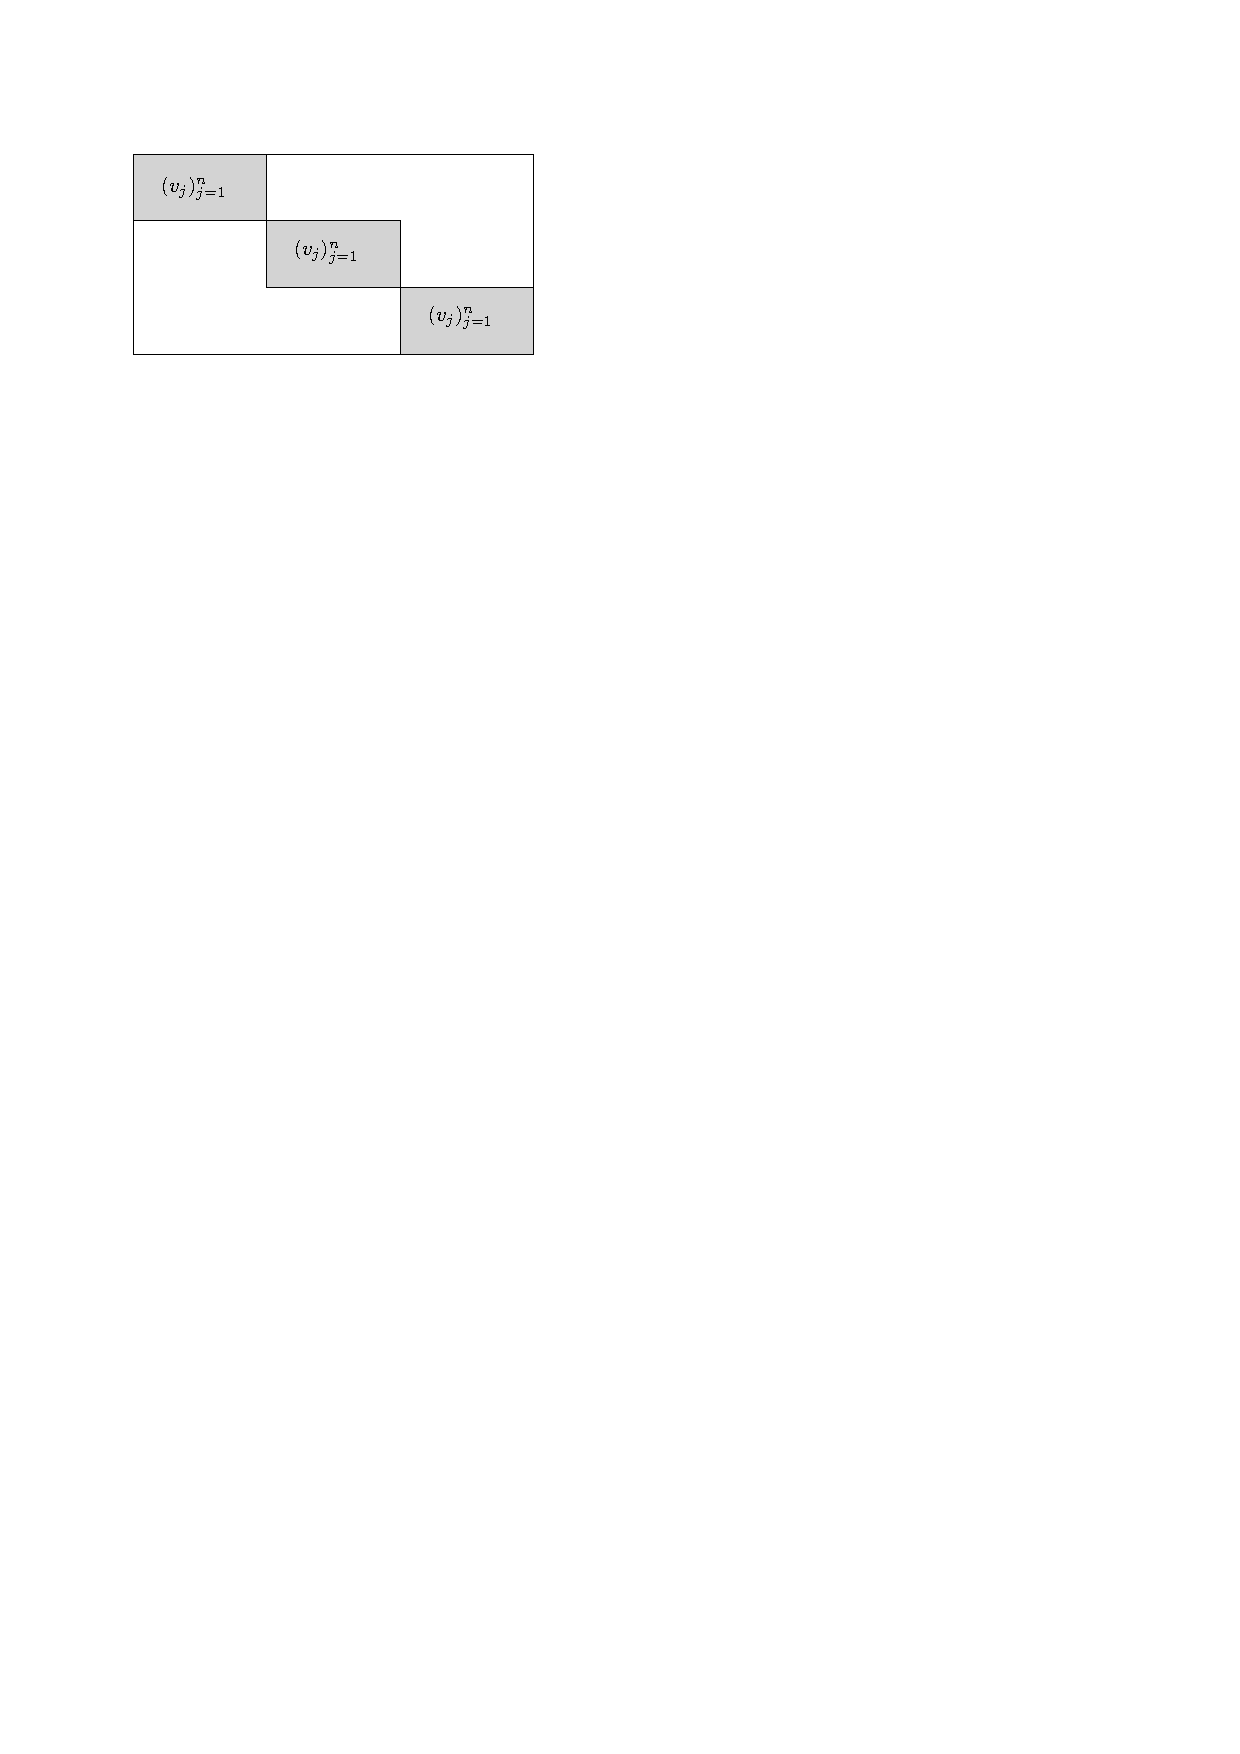
\includegraphics{cloning}
  \caption{The block structure of $(v_{\ell,j})_{\ell,j}$ for
    $d = 3$. All unshaded entries are $0$'s. }
  \label{fig:ch6a-cloning}
\end{figure}

% Let $e_1,\ldots,e_m$ be the standard basis for $\R^m$, so that
%  $v_j = \sum_i v_j(i) e_i$ for $j$ in $[n]$. 
%  We create $r$ disjoint copies of the instance as follows.
%  For each $e_i$, create $r$ distinct coordinates $e_{i,\ell}$, one for each $\ell\in [r]$.
%  We view 
%  %$\{e_{1,\ell},\ldots,\e_{m,\ell}\}$ as the $\ell$-th copy of $\R^m$, and 
%  the $\{e_{i,\ell}\}_{i\in [m],\ell  \in [r]}$ as forming the standard basis of $\R^{rm}$. 
% For each $v_j \in [n]$, create $r$ copies $v_{j,\ell}=\sum_i v_j(i) e_{i,\ell}$ of $v_j$ (on different sets of coordinates), one for each $\ell\in [r]$. So each $v_{j,\ell}  \in \R^{rm}$ and $\|v_{j,\ell}\|_2 = \|v_j\|_2 \leq 1$.
%Then $\tilde{B}$ corresponds to matrix with rows $e_{i,\ell}$ and columns $v_{j,\ell}$.

Consider now the convex body  $K = \cap_{i=1}^m K_i$ in $\R^{dm}$ defined by the intersection of the bodies
\[K_i=\{ y\in \R^{dm} :  \sum_{\ell=1}^d y(\ell,i)^2 \leq 2d\},\]
where we use $y(\ell,i)$ as shorthand for $y((\ell-1)m + i)$. In other
words, we think of vectors in $\R^{dm}$ as having $d$ blocks of
$m$ coordinates each, and $y(\ell, i)$ is the $i$-th coordinate in the
$\ell$-th block.
We claim that $K$ has large Gaussian measure.
\begin{claim} 
  For $d \lesssim \log(2m)$ large enough,  $\gamma^{dm} (K) \geq 1/2$.   
\end{claim}
\begin{proof}
  As $K = \cap_{i=1}^m K_i$, by the union bound it suffices to show
  that $\gamma^{dm} (\R^{dm} \setminus K_i ) = \Pr[ \sum_{\ell=1}^d
  \grv(\ell,i)^2 > 2 d] \leq 1/2m$,  where the $g(\ell,i)$ are
  independent standard Gaussian random variables.

  For each $i$ and $\ell$, we have $\E[g(\ell,i)^2]=1$ and $g(\ell,i)^2$ has subexponential tails, and thus by %i.e.,~$\Pr[g^2 \geq t] \leq  c_1\exp(-c_2t)$ for some fixed $c_1,c_2>0$.
 standard tail bounds, \eg, \cite[Corollary 2.8.3]{vershynin}, we have
%\begin{equation}
 % \label{eq:conc-subexp}
 \[\Pr\Big[\sum_{\ell=1}^d g(i,\ell)^2   \geq (1+\eps) d \Big]  \leq  2\exp(- cd \min (\eps,\eps^2)),\]
%\end{equation} 
for some fixed $c>0$. Plugging $\eps=1$, $d \ge \frac{1}{c}
\ln(4m)$ gives the result.
\end{proof}
Consider the coloring $x' \in \{-1,1\}^{dn}$
obtained by applying Theorem \ref{thm:bana}
to the $dn$ vectors $v_{\ell,j}$ and the body $K$. Let us use
$x'(\ell,j)$ for the color (\ie, value in $\{-1, +1\}$) given to
$v_{\ell,j}$.  Let $y$ denote the
resulting discrepancy vector $\sum_{\ell=1}^d\sum_{j = 1}^n x'(\ell,j)
v_{\ell,j}$.
 Then $\frac{1}{5} y \in K$, and, by the definition of $K$, we have
 that  $\frac{1}{5} y \in K_i$ for each $i\in [m]$. Thus, $\sum_{\ell=1}^d y(\ell,i)^2 \leq 10 d$.
 Also notice that, as $v_{\ell,j}(\ell,i) = v_{j}(i)$ for each $\ell$,
 and $v_{\ell,j}(\ell',i) = 0$ whenever $\ell \neq \ell'$, the entries of $y$ are
\[  y(\ell,i)  = \sum_{j=1}^n x'(\ell,j) v_{\ell,j}(\ell,i) =  \sum_{j=1}^n x'(\ell,j) v_{j}(i).\]
This gives us that
\begin{equation}
\label{eq:cloning-trick-bound}
\sum_{\ell=1}^d \Big(\sum_{j=1}^n x'(\ell,j) v_{j} (i)\Big)^2 =
\sum_{\ell=1}^d y(\ell,i)^2  \leq 50 d.
\end{equation}
%we have that 
Consider the vector coloring $x:[n] \to \R^d$ with vectors
\[x(j) \eqdef \frac{1}{\sqrt{d}} (x'(1,j),\ldots,x'(d,j)) \qquad \text{ for $j \in [n]$}.\]
Clearly, $\|x(j)\|_2=1$ as each $x'(\ell,j)$ is in $\{-1,+1\}$. 
Moreover, for each $i\in [m]$, the vector discrepancy is at most  
    \begin{align*}
      \bigg\| \sum_{j=1}^n x(j) v_j(i) \bigg\|_2^2
      & = \frac{1}{d} \sum_{\ell=1}^d \Big( \sum_{j=1}^n x'(\ell,j) v_j(i)\Big)^2   = \frac{1}{d} \sum_{\ell=1}^d  y(\ell,i)^2 \leq 10,  %\tag{ by \eqref{eq:cloning-trick-bound}}
         \end{align*}
   where the last two steps follow from \eqref{eq:cloning-trick-bound}.
\end{proof}

Let us mention another equivalent view of
Theorem~\ref{thm:komlos-vec-disc}. Instead of defining the vectors
$x(j) = \frac{1}{\sqrt{d}} (x'(1,j), \ldots, x'(d,j))$, we think of
$x'$ as defining a random coloring. In particular, we can set
$x(j) \eqdef x(\ell,j)$, where $\ell \in [d]$ is chosen uniformly at
random. Then the proof of Theorem~\ref{thm:komlos-vec-disc} shows that
\begin{equation}\label{eq:ch6a-veckomlos-rand}
  \max_{i = 1}^m \E\Big(\sum_{j} x(j) v_j(i)\Big)^2 \lesssim 1.
\end{equation}

Theorem~\ref{thm:komlos-vec-disc} in fact holds with the implied constant on the right hand side of \ref{eq:komlos-vec-disc} equal to $1$, which is clearly best possible. We give a different proof of a more general version of this better upper bound in Chapter~\ref{ch:online}. 

\section{The Main Geometric Core}
\label{sec:bana-core}
The original proof of Theorem \ref{thm:bana} by Banaszczyk was non-algorithmic and based on clever convex geometric argument and properties of Gaussian measures. 
The main technical core of his proof is the following geometric fact. See also Figure \ref{fig:bana:kstar}.
\begin{theorem}
\label{thm:bana-star}
For any convex body $K \in \R^m$ with $\gamma^m(K) \geq 1/2$ and any vector $u \in \R^m$ with $\|u\|_2 \leq 1/5$, there is a convex body 
$K*u$ contained in $(K-u) \cup (K+u)$ such that $\gamma^m(K*u) \geq \gamma^m(K)$. 
\end{theorem}

\begin{figure}[hbtp!]
    \centering
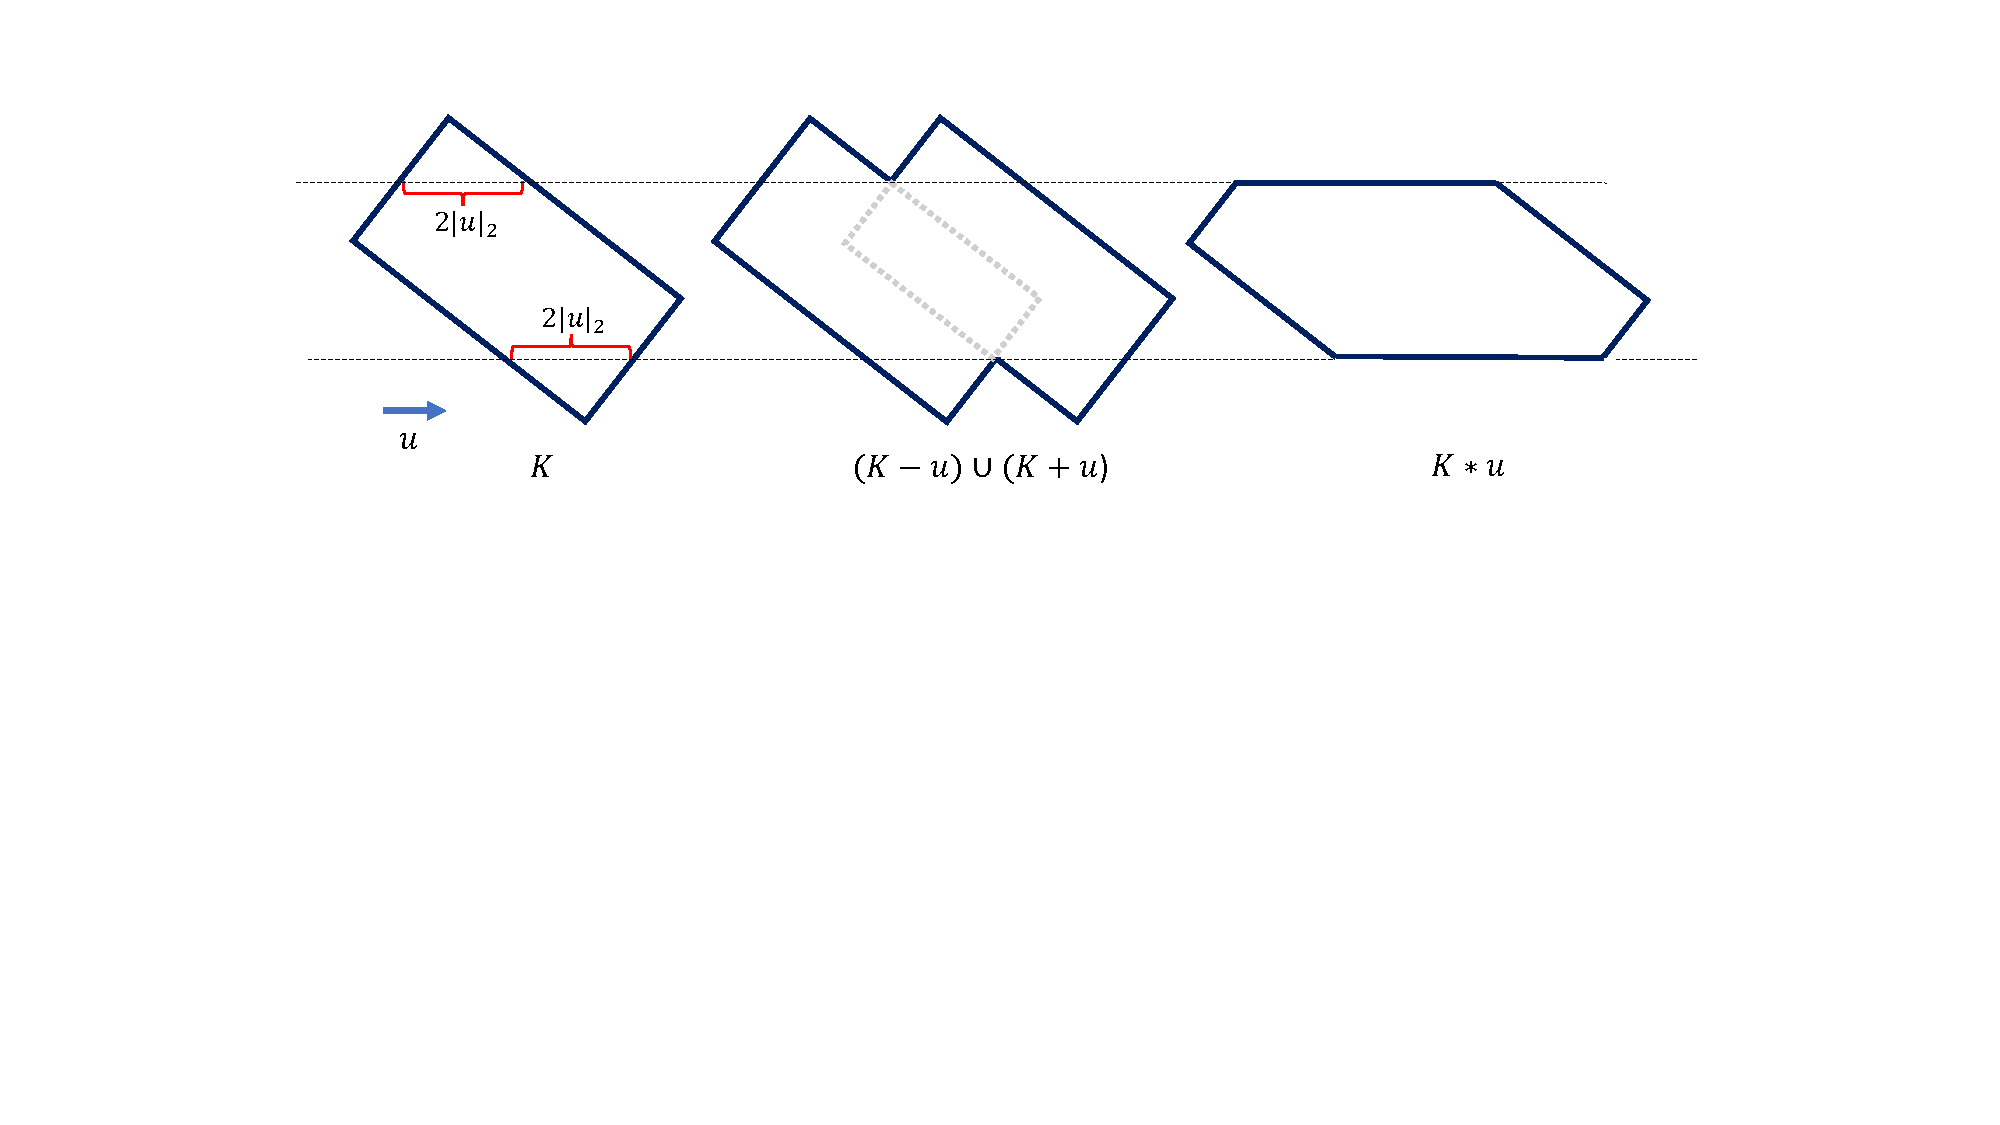
\includegraphics[scale=0.5, trim={3mm 2mm 2mm 3mm}]{bana-figures/figure-bana-1.pdf}
    \caption{The body $K*u$ obtained from $K$.}
    \label{fig:bana:kstar}
\end{figure}

% Theorem  \ref{thm:bana-star} is the main technical core of Banaszczyk's result and its proof involves several beautiful ideas. 
% In particular, Banaszczyk uses an elegant and powerful idea of Ehrhard symmetrization to reduce computations involving Gaussian measure of $m$-dimensional bodies to those involving Gaussian measure of one dimensional intervals!
Chapter \ref{ch:bana-proof} will be devoted entirely to the proof of Theorem \ref{thm:bana-star}.
For now, it does not matter how the body $K*u$ is obtained, and let us see how Theorem \ref{thm:bana} follows directly from Theorem \ref{thm:bana-star}. 
\begin{proof}(Theorem \ref{thm:bana}).
We apply induction on the number of vectors $n$.

The base case of $n=0$ holds as the origin $\mathbf{0}$ is
in $K$. Indeed, if $\mathbf{0} \notin K$, then, because $K$ is convex
and closed,
there must be a hyperplane $h$ separating $\mathbf{0}$ and $K$, \ie,
there is some $y \in \R^m$ and $\alpha < 0$ such that $\ip{x,y} \le  \alpha$ for all $x \in
K$ (this is the hyperplane separator theorem, see~\cite[Corollary~11.4.2]{Rockafellar}). However,
\[
\gamma^m(K) \le \gamma^m(\{x\in \R^m: \ip{x,y} \le \alpha\}) =
\Pr[\ip{\grv,y} \le \alpha] < \frac12,
\]
for a standard Gaussian random vector $\grv \in \R^m$, contradicting
the assumption $\gamma^m(K) \geq 1/2$.

Suppose the result holds for $n-1$.
Consider the convex body $K'=K*v_n$. Then $\gamma^m(K') \geq 1/2$ by Theorem \ref{thm:bana-star}, and  
by the inductive hypothesis %on $v_1,\ldots,v_{n-1}$ and $K'$,
there exist signs $x_1,\ldots,x_{n-1} \in \{-1,1\}$ such that 
$u := x_1 v_1 + \cdots + x_{n-1} v_{n-1} \in K'$. Now as $K' \subseteq (K-v_n) \cup (K+ v_n)$, 
either $u \in K-v_n$ in which case we set $x_n=1$ so that 
$x_1v_1+ \ldots + x_{n-1}v_{n-1} + x_n v_n =  u+ v_n \in K$, or, otherwise
$u \in K+v_n$ and we can set $x_{n}=-1$.
% must lie in at least one of $K-v_n$ or  $K+v_n$. In the first case, we can set $x_n=1$ so that signs satisfy $x_1v_1+ \ldots + x_{n-1}v_{n-1} + x_n v_n =  u+ v_n \in K$. Similarly, in the second case we can set $x_{n-1}=-1$
% so that  $x_1v_1+ \ldots + x_{n-1}v_{n-1} + x_n v_n =  u- v_n \in K$.
\end{proof}
Despite the simplicity of this inductive argument, it is unclear
how to use it to obtain an efficient algorithm to find the
coloring $x$. In general, a convex body $K$ can be very complicated
and require exponential size to describe it in any reasonably accurate
way. Even if the initial body $K$ is simple (like the unit
cube or the Euclidean ball), a few applications of the $*$ operator
above might, potentially, make it very complicated. In particular,
there is no known way to construct an efficient membership oracle for
the intermediate bodies in the inductive proof of
Theorem~\ref{thm:bana} above using a membership oracle for the initial $K$.

%This result is described in Theorem \ref{}.
%  In Section \ref{}, we discuss some further surprising applications of Banaszczyk's result.
 
%  \section{Using Theorem \ref{thm:bana-star}}

% We show how Theorem \ref{thm:bana} follows from Theorem \ref{thm:bana-star}.

%We remark that Theorem \ref{} does not require $K$ to be symmetric.


%\section{Sub-Gaussian Distribution over Discrepancy Vectors}
\section{Equivalence to Sub-Gaussianity}
\label{sec:bana-subgaussian}
Recall that a Gaussian random variable $\grv$ with mean $0$ and
variance $\sigma^2$ has a  moment generating function
$ \E[\exp(\lambda \grv)] = \exp(\lambda^2 \sigma^2/2)$ for all $\lambda
\in \R$. This property motivates the following (standard) definition.

\begin{definition}[sub-Gaussian Random Variable]
We say that a mean $0$ real-valued random variable $X$ is $\sigma$-\df{sub-Gaussian} if  
\[ \E[ \exp(\lambda X)] \leq \exp(\sigma^2 \lambda^2/2) \quad \text{for all $\lambda \in \R$}.\]  
\end{definition}
As the name suggests, if $X$ is $\sigma$-sub-Gaussian then it has sub-Gaussian tails.\footnote{Sometimes in the literature, this property is referred to $\sigma^2$-sub-Gaussian instead, but we use $\sigma$-subguassian throughout the text.} Indeed, setting $\lambda = t/\sigma^2$ above and applying Markov's inequality gives that for any $t>0$,
\begin{align*}\Pr[ X \geq t] &  \le \inf_{\lambda \ge 0} \Pr[\exp(\lambda X)  \geq
  \exp(\lambda t)] \\ 
  & \leq \inf_{\lambda \ge 0} \exp(\lambda^2 \sigma^2/2 - \lambda t) = \exp(-t^2/2\sigma^2).\end{align*}
Notice that if $X_1,\ldots,X_n$ are independent and $X_i$ is $\sigma_i$-sub-Gaussian with mean-zero, the sum $X = \sum_i X_i$ is $\left(\sum_i \sigma_i^2\right)^{1/2}$-sub-Gaussian as
\[ \E\exp(\lambda X) = \prod_i \E[\exp(\lambda X_i)] \leq \prod_i \exp(\sigma_i^2 \lambda^2/2).\]
Also, any $X$ distributed on $[-c,c]$ with mean-zero is
$c$-sub-Gaussian: this result is also known as Hoeffding's lemma.

The definition above is extended to random vectors by asking that each
one-dimensional marginal is sub-Gaussian.

\begin{definition}[sub-Gaussian Random Vector] A vector valued random
  variable $X \in \R^m$ with mean $0$ is $\sigma$-sub-Gaussian if for all vectors $x \in \R^m$, we have that  
\[ \E \exp( \ip{X,x})] \leq \exp(\sigma^2 \|x\|^2/2).\]
Equivalently, the projection $\ip{X,\theta}$ of $X$ in any direction
$\theta$, $\|\theta\|_2 = 1$ is a $\sigma$-sub-Gaussian real-valued
random variable.  
\end{definition} 

\paragraph{An equivalent version of Banaszczyk's Theorem.}
Surprisingly,  Theorem \ref{thm:bana} 
%and \ref{thm:bana-sub-Gaussian} 
is equivalent (up to various $O(1)$ factors) to a statement that does not involve mentioning any convex body $K$.

% Notice that Theorem \ref{thm:bana-sub-Gaussian} does not involve any convex body $K$, which makes it much more amenable to designing efficient algorithms. We will describe this in detail in Chapter \ref{}.


%is symmetric, that is $K=-K$. This is almost without loss of generality, because for any arbitrary body $K$ with $\gamma_m(K)\geq 3/4$, the body $K'= K \cap (-K)$ is symmetric and has Gaussian measure at least $1/2$ as $\gamma_m(\overline{K'}) \leq \gamma_m(\overline{K}) +\gamma_m(\overline{-K}) \leq 1/4 + 1/4 =1/2$. As $K' \subset K$ we can work with $K'$.
% An interesting consequence of Theorem \ref{} is the following.
Consider the following statement.
\begin{theorem}
\label{thm:bana-subgaussian}
    Given arbitrary vectors $v_1,\ldots,v_n \in \R^m$ with $\|v_j\|_2
    \leq 1$ for every $j \in [n]$, there is a probability distribution
    $D$ over colorings $x \in \{-1,1\}^n$ such that the discrepancy
    vector $Y \eqdef \sum_{j=1}^n x(j) v_j$ is $O(1)$-sub-Gaussian
    when $x$ is sampled according to $D$.
\end{theorem}

It turns out that Theorems~\ref{thm:bana}~and~\ref{thm:bana-subgaussian} are equivalent up to constant factors. We sketch the argument below.
%This was shown by \cite{DGLN16}, motivated by the question of finding an efficient algorithm for Theorem \ref{}.
% Notice that Theorem \ref{thm:bana-subgaussian} does not involve any convex body $K$, which makes it much more amenable to designing efficient algorithms. We will describe this in detail in Chapter \ref{}.

To show that Theorem \ref{thm:bana} implies Theorem~\ref{thm:bana-subgaussian} one can
 use a cloning trick similar to that in Section~\ref{sec:komlos-sdp-bound}.
The idea is to make multiple copies of the instance and apply Theorem
\ref{thm:bana} with a suitably defined convex body $K$, and view the
uniform distribution on the colorings for these copies as the
distribution $D$. This is similar to the alternative view of
Theorem~\ref{thm:komlos-vec-disc} above, but, instead of asking for
the second moment bound \eqref{eq:ch6a-veckomlos-rand}, we ask that
the random vector $\sum_{j = 1}^n x(j) v_j$ is $O(1)$-sub-Gaussian. 
The details of showing this are analogous to the proof of
Theorem~\ref{thm:komlos-vec-disc}, but are more involved, as one needs
to make exponentially many copies. We refer to \cite{rothvoss-online} for details.
%\footnote{It is a standard fact that the support of any $O(1)$-sub-gaussian random vector in $\R^m$ must be exponentially large in $m$.} 


The reverse implication will be more relevant for us, since we will
use it to give an algorithm for Theorem~\ref{thm:bana} in Chapter
\ref{ch:gram-schmidt}. In particular, we will show that a
distribution $D$ satisfying Theorem~\ref{thm:bana-subgaussian} can be
sampled efficiently.

 Intuitively, Theorem \ref{thm:bana-subgaussian} should imply Theorem \ref{thm:bana} because 
 the random vector $Y$ in Theorem \ref{thm:bana-subgaussian} is $O(1)$ sub-Gaussian, and as $\gamma^m(K)\geq 1/2$, a standard Gaussian $\grv \in \R^m$ lies in $K$ with probability at least $1/2$.
So $Y$, being ``more concentrated'' than a Gaussian with variance
$O(1)$ in every direction, should also lie in some $O(1)$-factor scaling of $K$ with
constant probability. 

While this intuition can be made rigorous, a
significant hurdle is that the definition of a sub-Gaussian random
vector only requires that the one-dimensional marginals are
sub-Gaussian, and does not make any requirements about
higher-dimensional marginals. Nevertheless, the following comparison
theorem, which is a deep result of Talagrand, allows us to get around
this obstacle. We refer to Talagrand's book~\cite{Talagrand-book} for
a proof; see also~\cite[Section 8.6]{vershynin}.

\begin{theorem}[Talagrand's Comparison Theorem]\label{thm:ch6a-talagrand}
  For any bounded set $T \subseteq \R^m$, and any $\sigma$-sub-Gaussian
  random vector in $\R^m$, we have
  \[
    \E \sup_{t \in T} \ip{X,t} \lesssim \sigma \,\,  \E\sup_{t \in T}
    \ip{\grv, t},
  \]
  where $\grv$ is a standard Gaussian random vector. 
\end{theorem}

To use Theorem~\ref{thm:ch6a-talagrand}, we need the notion of a polar set, defined for a set $K
\subseteq \R^m$ by
\[
  K^\circ \eqdef \{y \in \R^m: \ip{x,y} \le 1 \,\,\,\, \forall x \in K\}.
\]
As a consequence of the hyperplane separator theorem, when $K$ is convex, closed, and
contains $0$, $K^{\circ \circ} = K$~\cite[Chapter 5]{Matousek-discgeom}. 

We give the main implication next. To avoid some technicalities, we
consider only the case where $\gamma^m(K)\geq 3/4$. This does not make
a difference for most applications of Theorem~\ref{thm:bana}.


% Let $K$ be a convex body such that the ball $B(0,r)$ of radius $r$ centered at the origin lies in $K$.  Then we have the following.
\begin{theorem}\label{thm:bana-subg-suff}
Suppose that the  random vector $Y$ in Theorem \ref{thm:bana-subgaussian}  is $\sigma$-sub-Gaussian.
There is a universal constant $c > 0$ such that, for any closed convex
set $K \subseteq \R^m$ containing $0$ with Gaussian measure $\gamma^m(K) \geq 3/4$, we have 
\[\Pr[ Y \in c\sigma K] \geq 1/2.\]
\end{theorem}
\begin{remark}
    Notice that if we could sample efficiently from the distribution $D$, then this also give an efficient algorithm to find a coloring $x$ with $\sum_j x_j v_j \in 2cc'K$, by sampling a couple of times from $D$.
\end{remark}
\begin{proof}%[Proof (Sketch)]
Let $B_{\ell_2^m}$ denote the unit $\ell_2^m$-ball. We claim that $\frac12
B_{\ell_2^m}\subseteq K$. Otherwise, there is a point $u$, $\|u\|_2 = \frac12$,
that is not in $K$, and, since $K$ is closed and convex, by the
hyperplane separator theorem there is a vector $y \in \R^m$ such that
$\ip{x,y} \le 1$ but $\ip{u,y} > 1$. By the Cauchy-Schwarz inequality,
$\ip{u,y} > 1$ implies $\|y\|_2 > 2$. Then, for the halfspace $H
\eqdef \{x \in \R^m: \ip{x,y} \le 1\}$ we have
\[
  \gamma^m(K) \le \gamma^m(H) = \Pr[\ip{\grv,y} \le 1] <
  \Phi(1/\|y\|_2) \leq \Phi(1/2) < 3/4.
\]
Above, $\grv$ is a standard Gaussian vector in $\R^m$, $\Phi$ is the
CDF of the one-dimensional standard Gaussian,  and we used the
fact that $\ip{\grv,y}$ is a one-dimensional Gaussian with mean $0$
and standard deviation $\|y\|_2 > 2$. This inequality contradicts
$\gamma^m(K) \ge 3/4$.

Using polarity, we have that $tK = \{x \in \R^m: \ip{x,y} \le t \
\forall y \in K^\circ\}$, for any $t \ge
0$. Theorem~\ref{thm:ch6a-talagrand} gives us 
\begin{equation}\label{eq:ch6a-comp}
  \E \sup_{z \in K^\circ} \ip{Y,z} \le c_1\sigma \E\sup_{z \in
    K^\circ} \ip{\grv,z}
\end{equation}
for a standard Gaussian random vector $\grv \in \R^m$ and some
absolute constant $c_1 >
0$. 

We want to show that $\E\sup_{z \in  K^\circ} \ip{\grv,z} \lesssim
1$. Since $\frac12 B_{\ell_2^m} \subseteq K$, the Cauchy-Schwarz theorem
implies that $K^\circ \subseteq 2B_{\ell_2^m}$, and the function
$f_K(x) \eqdef \sup_{z \in K^\circ} \ip{x,z}$
is $2$-Lipschitz with respect to the $\ell_2^m$ norm. (Note that $f_K$
is just the norm with unit ball $K$ when $K = -K$ and $K$ is bounded
and has nonempty interior.) Suppose, for contradiction, that
$\E[f_K(\grv)] > C$ for some sufficiently large constant $C > 1$. Then, the
Gaussian concentration inequality~\cite[Corollary~8.6.2]{vershynin} gives us that, for
some absolute constant $c_2 > 0$,
\[
  \gamma^m(K) = \Pr[f_K(\grv) \le 1]
  \leq \Pr[f_K(\grv) \le \E[f_K(\grv)] - (C-1)] \le e^{-c_2 (C-1)^2}.
\]
Choosing $C$ sufficiently large contradicts $\gamma^m(K) \ge
\frac34$, so $\E\sup_{z \in  K^\circ} \ip{\grv,z} = \E[f_K(\grv)]
\le C$. Together with \eqref{eq:ch6a-comp}, this gives us
\(
\E \sup_{z \in K^\circ} \ip{Y,z}\le c_1C\sigma ,
\)
as well. 
Now, by Markov's inequality, $\sup_{z \in K^\circ} \ip{Y,z} \le 2c_1C\sigma$ with probability at
least $\frac12$,  and
therefore, $Y \in (2c_1 C)K$ with the same probability.
\end{proof}

It is not hard to extend Theorem~\ref{thm:bana-subg-suff} to \emph{symmetric} closed
convex sets $K$ with $\gamma^m(K) \ge \frac12$. The main observation
is that such a set $K$ still must contain a Euclidean ball of some
fixed constant radius $r$, since, if it did not, it would be
sandwiched between two hyperplanes of distance less than $2r$
apart. Extending the theorem to non-symmetric $K$ is, however,
non-trivial. For example, if $K$ is the halfspace $\{x \in \R^m: x(1)
\le 0\}$, then $\gamma^m(K) = \frac12$, but $K$ does not contain a
Euclidean ball of any positive radius around the origin, and its polar
set $K^\circ$ is unbounded, so $\E \sup_{z \in K^\circ} \ip{Y,z} =
\infty$. Nevertheless, it is possible to algorithmically reduce the
case of non-symmetric $K$ with $\gamma^m(K) \ge \frac12$ to the
symmetric case: we refer to~\cite{DGLN-journal} for the details.

\section{Prefix discrepancy}
In many applications of discrepancy, one might actually want to bound the discrepancy of every prefix sum, instead of just the overall sum $\sum_i x(i) v_i$. One example is the application to the Steinitz Problem in Section~\ref{sec:ch1-steinitz}, which we revisit later in this section.
The following result, also due to Banaszczyk, controls the discrepancy of every prefix sum, at the expense of a slight increase in the Gaussian measure of $K$. 
%In all the applications that we are aware of this do bounds over those 

%In  Banaszczyk \cite{B12} further extended this result to handle prefixes, using a clever inductive argument.
\begin{theorem}\label{thm:bana2}
 Given arbitrary vectors $v_1,\dots,v_n\in\mathbb{R}^m$ with $\|v_i\|_2 \leq 1/5$ and any
convex body $K\subseteq \mathbb{R}^m$ with $\gamma^m(K)\ge 1-1/(2n)$,
there exists a $\pm 1$ coloring $x$ such that $\sum_{j=1}^k x(j) v_j \in K$ for each $k\in [n]$.
\end{theorem}

Similarly to Theorem \ref{thm:bana}, this result also follows from Theorem \ref{thm:bana-star} based on a clever induction argument.  
\begin{proof}
Consider the convex bodies $K_n,K_{n-1},\ldots,K_1$ defined
iteratively as follows:  $K_n\eqdef K$ and $K_{j}\eqdef(K_{j+1}*v_{j+1}) \cap K$, for $j=n-1,\ldots,1$.  

We first show by backwards induction that $\gamma^m(K_j) \geq 1/2 + (j-1)/2n$. This implies that $\gamma^m(K_j) \geq 1/2$ for all $j\geq 1$.

The base case of $j=n$ holds as $\gamma^m(K_n) = \gamma^m(K) \ge 1-1/2n$.
Suppose the claim holds for some $j \leq n$. Then 
\begin{align*}\gamma^{m}(K_{j-1}) &  = \gamma^m((K_{j}*v_{j}) \cap
                                      K) \geq  \gamma^m(K_{j}*v_{j}) - \gamma^m(\R^m\setminus {K}) \\
& \geq    \gamma^m(K_{j})  - \gamma^m(\R^m\setminus{K}) \geq  \frac{1}{2} +\frac{j-1}{2n} -\frac{1}{2n} = \frac{1}{2} + \frac{ j-2}{2n},
\end{align*}
where we use that $\gamma^m(K_{j}*v_{j}) \geq \gamma^m(K_{j})$ as
$\gamma^m(K_{j}) \geq 1/2$ by Theorem \ref{thm:bana-star}, and that
$\gamma^m(\R^m \setminus {K})\leq 1/(2n)$.

We now show that any sequence $x(1), \ldots, x(k) \in \{-1,+1\}$ satisfying
$\sum_{j=1}^\ell x(j) v_j \in K_\ell$ for all $\ell \in [k]$, can be extended to
$x(1), \ldots, x(k+1) \in \{-1,+1\}$ such that $\sum_{j=1}^{k+1} x(j)
v_j \in K_{k+1}$. This will imply the result as the final sequence
$x(1),\ldots,x(n)$ will satisfy $\sum_{j=1}^k x(j) v_j \in K_k
\subseteq K$ for all $k\in [n]$.
%this will imply that each prefix sum $\sum_{i=1}^j x_i v_i$ of the final signing $x_1,\ldots,x_n$ will lie in $K$.

To initialize the sequence, we pick some $x(1)$ such that $x(1) v_1 \in K_1$. Such an $x(1)$ exists by Theorem \ref{thm:bana} as $\gamma^m(K_1) \geq 1/2$. 
Then, for $k\ge 1$, let $x(1),\ldots,x(k)$ be the sequence chosen so
far, and define $y_k\eqdef\sum_{j=1}^k x(j) v_j$.  Then
\[y_k\in K_k \subseteq K_{k+1}*v_{k+1} \subseteq (K_{k+1}+v_{k+1}) \cup
  (K_{k+1}- v_{k+1}),\] and at least one of $y_k+v_{k+1}$ or $y_k-v_{k+1}$ must lie in $K_{k+1}$. We set $x(k+1)$ accordingly and extend the sequence.
\end{proof}

It is possible to use the proof of Theorem~\ref{thm:bana2} and the
cloning trick in order to formulate a statement similar to
Theorem~\ref{thm:bana-subgaussian} for prefix sums. We state this
theorem next, and refer to the work of Kulkarni, Reis, and Rothvoss~\cite{rothvoss-online} for the
proof.
\begin{theorem}\label{thm:bana-prefix-subgaussian}
  Given arbitrary vectors $v_1,\ldots,v_n \in \R^m$ with $\|v_i\|_2
  \leq 1$, there is a distribution $D$ over colorings $x \in
  \{-1,1\}^n$ such that, for each $k \in [n]$, the prefix discrepancy
  vector $Y_k \eqdef \sum_{j=1}^k x(j) v_j$ is $O(1)$-sub-Gaussian when
  $x$ is sampled from $D$.
\end{theorem}

Unlike Theorem~\ref{thm:bana-subgaussian}, there is no known efficient
algorithm to sample from the distribution $D$. More generally, it is
an intriguing open problem how to make Theorem \ref{thm:bana2}
algorithmic. 

%Even though we require $\gamma^m(K) \geq 1-1/(2n)$ \ref{thm:bana2} in constrast to  $\gamma^m(K)\geq 1/2$ in Theorem \ref{thm:bana}, this does not typically lead to worse results.
\subsection{Prefix Koml\'os Problem and the Steinitz Lemma}
Theorem \ref{thm:bana2} directly implies the following bound for the prefix version of the Koml\'os problem.

\begin{theorem}[Prefix Koml\'os]\label{thm:prefix-komlos}
  Given vectors $v_1,\dots,v_n\in\mathbb{R}^m$ with $\|v_j\|_2 \leq 1$, 
  there exists a coloring $x:[n]\to\{-1,+1\}$ such that  $\|\sum_{j=1}^k x(j) v_j\|_2 \lesssim \sqrt{\log(2n)}$ for all $k\in [n]$. I.e., the signed series constant satisfies 
  \[
  \sser(B_{\ell_2^m},\ell_\infty^m,n) \lesssim \sqrt{\log(2n)}.
  \]
\end{theorem}
\begin{proof}
We apply Theorem~\ref{thm:bana2} with $K \eqdef [-t,t]^m$ and $t>0$ such
that  \[\gamma^m(K) \geq 1-1/2n.\]  As in the proof of
Theorem~\ref{thm:komlos-bana}, we see that setting $t \lesssim \sqrt{\log(2mn)}$ suffices.
By Remark \ref{rem:bana-komlos-trick}, we can also assume that $m\leq n^2$.
\end{proof}

A similar proof shows the following bound, which gets tantalizingly
close to resolving Problem~\ref{prob:steinitz} for the case of the
Euclidean norm.

\begin{theorem}\label{thm:sser-ellp}
  Let $p \ge 2$ and suppose that the vectors $v_1, \ldots, v_n \in
  \R^m$ each satisfy $\|v_j\|_2 \le 1$. There exists a coloring $x:[n]
  \to \{-1,+1\}$ such that $\|\sum_{j=1}^kx(j)v_k\|_p \lesssim
  \sqrt{p}m^{1/p} + \sqrt{\log n}$. I.e., the signed series constant satisfies 
  \[
  \sser(B_{\ell_2^m},\ell_p^m,n) \lesssim \sqrt{p}m^{1/p} + \sqrt{\log n}.
  \]
\end{theorem}
\begin{proof}
  We apply Theorem~\ref{thm:bana2} with $K = tB_{\ell_p^m}$, where
  $B_{\ell_p^m}$ is the unit ball of the $\ell_p^m$ norm, and $t$ is
  chosen so that $\gamma^m(K) \ge 1 - 1/2n$. %Notice that, for
  %a standard Gaussian vector $\grv \in \R^m$, 
  By Jensen's inequality
  and standard bounds on the $p$-th moment of a
  Gaussian~\cite[Proposition 2.5.2]{vershynin}, we have
  \[
    \E[\|\grv\|_p] \le \E[\|\grv\|_p^p]^{1/p}
    = \E\left[\sum_{i=1}^m |\grv(i)|^p\right]^{1/p} \lesssim \sqrt{p}m^{1/p}.
  \]
  By the Gaussian concentration inequality, since $\|\cdot\|_p$ is
  1-Lipschitz with respect to the Euclidean norm when $p \ge 2$,
  \[
    \Pr[\|\grv\|_p > \E[\|\grv\|_p] + s] \le e^{-c s^2}
  \]
  for an absolute constant $c > 0$. Choosing $s \eqdef c'
  \sqrt{\log(2n)}$ for a large enough constant $c' > 0$ makes  the
  right hand side at most $\frac{1}{2n}$. Since the left hand side
  equals $\gamma^m(\R^m\setminus K)$ for $t = \E[\|\grv\|_p] + s
  \lesssim \sqrt{p}m^{1/p} + \sqrt{\log(2n)}$, this proves the lemma.
\end{proof}


If Theorem~\ref{thm:sser-ellp} could be improved by removing the
additive $\sqrt{\log 2n}$ term, then it would give tight bounds for
Problem~\ref{prob:steinitz} for any constant $p \ge 2$. In particular, via
Chobanyan's transference theorem (Theorem~\ref{thm:ch1-chobanyan}), it would imply
\[
  \st(B_{\ell_p^m}, \ell_p^m) \le m^{\frac12 - \frac1p}\st(B_{\ell_2^m}, \ell_p^m) 
  \le m^{\frac12 - \frac1p}\sser(B_{\ell_2^m}, \ell_p^m) 
  \lesssim \sqrt{pm},
\]
which is tight for constant $p \ge 2$. %Similarly, it would imply $\st(B_{\ell_p^m}, \ell_p^m) \lesssim m^{1/p}$ for $p \in [1,2]$.

%In addition to sharpening , 
Another open
problem is to make Theorem~\ref{thm:sser-ellp} or Theorem~\ref{thm:prefix-komlos},
algorithmic. For both theorems, there is no known efficient algorithm to find
the coloring $x$ given the vectors $v_1, \ldots, v_n$.

% It is an intriguing open how to make Theorem \ref{thm:bana2} algorithmic, even for the special case of the Prefix Koml\'os problem.
% As in Th
% Theorem \ref{thm:bana2} is equivalent to the following statement
% There is a distribution $D$ on colorings $x \in \{-1,1\}^n$ such that for every $j \in [n]$, the sum $\sum_{i=1}^j x_j v_j$ is $O(1)$-sub-gaussian, when $x$ is sampled from $D$.

% One approach to make it algorithm would be design an algorithm which samples a coloring from such a distribution.


\subsection{Prefix Discrepancy and the $\gamma_2$ Norm}

Theorem~\ref{thm:bana2} also immediately implies that
Lemma~\ref{lm:fact-ub} can be extended to bound prefix discrepancy, at
the cost of a small increase in the logarithmic factor. Here we recall
that the prefix discrepancy of an $m\times n$ real matrix $\mat = (w_i)_{i=1}^n$ is
the quantity
\[
  \pdisc((w_i)_{i = 1}^n) \eqdef
  \min_{\col:[n]\to\{-1,+1\}}\max_{j=1}^n \left\|\sum_{i = 1}^j\col(i)w_i \right\|_\infty.
\]
This definition coincides with our definition of
$\pdisc_{\ell_\infty^m}$ from Chapter~\ref{ch1-intro}.


\begin{lemma}\label{lm:fact-ub-prefix}
  For any $m\times n$ matrix $\mat$ 
  we have
  \[
  \pdisc(\mat) \lesssim \gamma_2(\mat) \sqrt{\ln(2mn)}.
  \]   
\end{lemma}
\begin{proof}
  By the definition of $\gamma_2(\mat)$, we need to show  that if $\mat$ can be written as the matrix
  product $\mat = UV$ of two matrices $U \in \R^{m\times k}$ and $V\in
  \R^{k\times n}$, where each row
  $u_i$ of $U$ satisfies $\|u_i\|_2 \le r$, and each column $v_j$ of
  $V$ satisfies $\|v_j\|_2 \le c$, then $\pdisc(\mat) \lesssim rc\sqrt{\ln(2mn)}$.
  Similarly to the proof of Lemma~\ref{lm:fact-ub}, we define the convex body
  \[
    K = \{ y \in \R^k: \|Uy \|_{\infty} \leq r\sqrt{2\ln{(2mn)}}  \}.
  \]
  Arguing as in the proof of Lemma~\ref{lm:fact-ub},
  we have $\gamma^m(K) \ge 1 - \frac{1}{2n}$.
  Now Theorem~\ref{thm:bana2} applied to the columns $\frac{1}{5c}v_1,
  \ldots, \frac{1}{5c}v_n$ of $\frac{1}{5c}V$ implies the lemma.
\end{proof}

In Chapter~\ref{ch:gamma2} we will use Lemma~\ref{lm:fact-ub-prefix}
to prove the best known upper bound for Tusn\'ady's problem (Problem~\ref{prob:tusnady}).

\section{Bibliographic Notes}

Theorems~\ref{thm:bana}~and~\ref{thm:komlos-bana} are due to Banaszczyk \cite{Bana98}. The
original proof was non-algorithmic and based on deep results from convex geometry. We will describe Banaszczyk's proof in detail in
Chapter \ref{ch:bana-proof}. 

Lemma~\ref{lm:fact-ub} is implicit in Larsen's work on data structure
lower bounds~\cite{disc-larsen}, and was made explicit by
Matou\v{s}ek, Nikolov, and Talwar~\cite{MNT}. 

The cloning trick in Section \ref{sec:komlos-sdp-bound} is due to
unpublished work by Shachar Lovett, Raghu Meka, and Oded
Regev. Nikolov~\cite{nikolov2013komlos} gave a different and direct proof of
Theorem~\ref{thm:komlos-vec-disc} where the implied constant on the
right hand side of \eqref{eq:komlos-vec-disc} is equal to $1$. Yet another proof of Theorem~\ref{thm:komlos-vec-disc}, also with the constant $1$ on the right hand side, was given by Dadush, Garg, Lovett, and Nikolov~\cite{DGLN16}.
Interestingly, it is unclear how to show this tight
bound using the cloning trick, as the body $K$ in
Theorem~\ref{thm:bana} needs to be scaled by $5$ if the vectors $v_j$
have unit length. We give another (previously unpublished) proof of the tight upper bound in Chapter~\ref{ch:online}.

The equivalence between
Theorems~\ref{thm:bana}~and~\ref{thm:bana-subgaussian} was shown by
Dadush, Garg, Lovett and Nikolov \cite{DGLN16}, motivated by the
question of finding an efficient algorithm for Theorem
\ref{thm:bana}. A direct proof of Theorem \ref{thm:bana-subgaussian},
and an efficient sampling algorithm for the distribution $D$, were given
later by Bansal, Dadush, Garg and Lovett~\cite{BansalDGL19} using an algorithm called the Gram-Schmidt Walk. We will
describe this algorithm and its analysis in detail in Section~\ref{ch:gram-schmidt}.

The argument we present here that Theorem \ref{thm:bana} implies
Theorem \ref{thm:bana-subgaussian} via the cloning trick is
different from the Dadush, Garg, Lovett, and Nikolov argument, which
was based on the minimax theorem.  The cloning trick based argument
for
Theorems~\ref{thm:bana-subgaussian}~and~\ref{thm:bana-prefix-subgaussian}
appears in unpublished work of Nikolov. Kulkarni, Rothvoss and Reis
apply a similar argument to prove that the sequence of signs can even
be computed online, albeit via an inefficient
algorithm~\cite{rothvoss-online}. We consider online algorithms for
discrepancy minimization in more detail in Chapter~\ref{ch:online}.

Theorem \ref{thm:bana2} for prefix discrepancy, and
Theorem~\ref{thm:prefix-komlos} for the prefix Koml\'os problem are
also due to Banaszczyk, in a more recent work~\cite{B12}. An intriguing open problem is to
find an efficient algorithmic version of either theorem. The
best known algorithmic bound in the prefix setting is $O(\log mn)$, which
remarkably also works in the online
setting~\cite{alweiss2020discrepancy}, and is based on a beautiful algorithm called the Self-Balancing Walk, that we will describe in detail
in Chapter \ref{ch:online}.  See also \cite{rothvoss-online,
  ChewiGRT22, LiuSS22} for related progress. 
  Finally, we remark that an algorithmic
$O((\log mn)^{1/2})$ discrepancy bound for the prefix Koml\'{o}s
problem would already be interesting to obtain in the special case
where each vector $v_i$ has only two non-zero entries, as it would
have implications for approximation algorithms for scheduling
problems~\cite{BansalRS22}.


% For prefix Komlos, the best algorithmic bound we know is $O(\log n)$
% (this can be done  in two ways: (i) using partial coloring method,
% or (ii) by writing an SDP with vector discrepancy $O(1)$ as in Section \ref{sec:komlos-sdp-bound}, and using the random walk based approach in Chapter \ref{}).  






% Can get both sub-gaussianity 

% \subsection{Exercises}
% Exercise. Show that for the Komlos problem we can assume that $m\leq n^2$. 

% Solution. Consider the  $m\times n$ matrix $A$ with columns $v_j$ and let $a_i$ denote its rows. As $\|v_j\|_2\leq 1$ for each $j$, and using that $\|a\|_1 \leq \|a\|_2 \sqrt{n}$ for any $a\in \R^n$ we have,
% \[n \geq \sum_{j=1}^n \|v_j\|_2^2 = \sum_{i=1}^m \|a_i\|_2^2 \geq  \|a_i\|_1^2/n,\]
% %by the Cauchy-Schwartz inequality.
% So all except at most $n^2$ rows satisfy $\|a_i\|_1 \leq 1$ and can be ignored and they can have discrepancy at most $1$ for any signing.


%%% Local Variables:
%%% mode: latex
%%% TeX-master: "book"
%%% End:
